   \section{General TrickHLA Configuration}

   \begin{frame}
      \frametitle{General TrickHLA Configuration}
      \begin{center}
      \Huge{General TrickHLA Configuration}
      \end{center}
   \end{frame}
   
   \begin{frame}
      \frametitle{General TrickHLA Configuration}
      General TrickHLA configuration consists of the following:
      \begin{enumerate}
         \item General TrickHLA Configuration
         \item Initializing the Federate
         \item Initializing the List of Known Federates
         \item Initializing the Debug Level (Optional)
         \item Initializing the Data Objects
         \item Initializing the Data Object Attributes
      \end{enumerate}
   \end{frame}
   
   \begin{frame}[fragile]
      \frametitle{General TrickHLA Configuration}
      \framesubtitle{Initializing the Central RTI Component Settings}
      \begin{itemize}
         \item The Pitch Central RTI Component (CRC) is initialized by specifying
         the host, port, and lookahead time as shown below. The host and port
         describe where the CRC is/will be running.
         \item Notice the settings are based on the simulation object name and
         the parameter name as they exist in the \texttt{S\_define} file.
         \item In the \texttt{RUN\_a\_side/input.py} file:
      \end{itemize}
\begin{Verbatim}[frame=single, fontsize=\footnotesize]
# Configure the CRC for the Pitch RTI.
THLA.federate.local_settings = "crcHost = localhost\n crcPort = 8989”
THLA.federate.lookahead_time = 0.25  # this is THLA_DATA_CYCLE_TIME
\end{Verbatim}
   \end{frame}
   
   \begin{frame}[fragile]
      \frametitle{General TrickHLA Configuration}
      \framesubtitle{Initializing the Federate}
      \begin{itemize}
         \item The input.py file settings determine how each federate shares data.
\begin{Verbatim}[frame=single, fontsize=\footnotesize]
In the RUN_a_side/input.py file:
THLA.federate.name                  = "A-side-Federate"
THLA.federate.enable_FOM_validation = False
THLA.federate.FOM_modules           = 
   "S_FOMfile.xml,TrickHLAFreezeInteraction.xml"
THLA.federate.federation_name       = "SineWaveSim"
THLA.federate.time_regulating       = True
THLA.federate.time_constrained      = True
\end{Verbatim}
         \item In the \texttt{RUN\_p\_side/input.py} file:
\begin{Verbatim}[frame=single, fontsize=\footnotesize]
THLA.federate.name                  = "P-side-Federate"
THLA.federate.enable_FOM_validation = False
THLA.federate.FOM_modules           = 
   "S_FOMfile.xml,TrickHLAFreezeInteraction.xml"
THLA.federate.federation_name       = "SineWaveSim"
THLA.federate.time_regulating       = True
THLA.federate.time_constrained      = True
\end{Verbatim}
      \end{itemize}
   \end{frame}
   
   \begin{frame}[fragile]
      \frametitle{General TrickHLA Configuration}
      \framesubtitle{Initializing the List of Known Federates}
      \begin{itemize}
         \item A list of federates known to be in the federation is initialized next.
         \item The simulation will wait for all federates designated as “required”
         to join the simulation before continuing on. These required federates
         define the distributed simulation parts that MUST exist for the
         simulation to run.
         \item In both the \texttt{RUN\_a\_side/input.py} and \texttt{RUN\_p\_side\_input.py} files:
\begin{Verbatim}[frame=single, fontsize=\footnotesize]
THLA.federate.enable_known_feds      = True
THLA.federate.known_feds_count       = 2
THLA.federate.known_feds             = trick.alloc_type(
   THLA.federate.known_feds_count, "TrickHLAKnownFederate" )
THLA.federate.known_feds[0].name     = "A-side-Federate"
THLA.federate.known_feds[0].required = True
THLA.federate.known_feds[1].name     = "P-side-Federate"
THLA.federate.known_feds[1].required = True
\end{Verbatim}
      \end{itemize}
   \end{frame}
   
   \begin{frame}[fragile]
      \frametitle{General TrickHLA Configuration}
      \framesubtitle{Initializing the Debug Level (Optional)}
      \begin{itemize}
         \item Although not required, it is recommended that you enable TrickHLA
         debug messages while you are getting your simulation to work with
         TrickHLA for the first time.
         \item Varying amounts of messages may be output by setting the debug
         level, which ranges from \texttt{THLA\_LEVEL0\_TRACE} (no messages) to
         \texttt{THLA\_LEVEL11\_TRACE} (all messages).
         \item For example:
\begin{Verbatim}[frame=single, fontsize=\footnotesize]
THLA.manager.debug_handler.debug_level = trick.THLA_LEVEL3_TRACE
\end{Verbatim}
      \end{itemize}
   \end{frame}
   
   \begin{frame}[fragile]
      \frametitle{General TrickHLA Configuration}
      \framesubtitle{Initializing the Data Objects}
      \begin{itemize}
         \item The TrickHLA data objects define the data the federates will exchange.
         \item For the sine wave simulation each federate will publish one
         object containing its own state data and will subscribe to the state
         data of the other federate (2 objects total).
         \item In both the \texttt{RUN\_a\_side/input.py} and \texttt{RUN\_p\_side\_input.py} files:
\begin{Verbatim}[frame=single, fontsize=\footnotesize]
THLA.manager.obj_count = 2
THLA.manager.objects   = trick.alloc_type( THLA.manager.obj_count,
   "TrickHLAObject” )
\end{Verbatim}
         \item The \texttt{S\_FOMfile.xml} FOM file defines the \texttt{Test} data class
         containing the following 8 attributes for the sine wave simulation:
         \textit{Name}, \textit{Time}, \textit{Value}, \textit{dvdt}, \textit{Phase},
         \textit{Frequency}, \textit{Amplitude}, and \textit{Tolerance}.
      \end{itemize}
   \end{frame}
   
   \begin{frame}[fragile]
      \frametitle{General TrickHLA Configuration}
      \framesubtitle{Initializing the Data Objects - RUN\_a}
      \begin{itemize}
         \item Data object configuration in the \texttt{RUN\_a\_side/input.py} file:
\begin{Verbatim}[frame=single, fontsize=\scriptsize]
# Configure the object this federate owns and will publish.
THLA.manager.objects[0].FOM_name            = "Test"
THLA.manager.objects[0].name                = "A-side-Federate.Test"
THLA.manager.objects[0].create_HLA_instance = True
THLA.manager.objects[0].attr_count          = 8
THLA.manager.objects[0].attributes          = trick.alloc_type(
   THLA.manager.objects[0].attr_count, "TrickHLAAttribute" )

# Configure the object this federate does not own and will subscribe to.
THLA.manager.objects[1].FOM_name            = "Test"
THLA.manager.objects[1].name                = "P-side-Federate.Test"
THLA.manager.objects[1].create_HLA_instance = False
THLA.manager.objects[1].attr_count          = 8
THLA.manager.objects[1].attributes          = trick.alloc_type(
   THLA.manager.objects[1].attr_count, "TrickHLAAttribute" )
\end{Verbatim}
      \end{itemize}
   \end{frame}
   
   \begin{frame}[fragile]
      \frametitle{General TrickHLA Configuration}
      \framesubtitle{Initializing the Data Objects - RUN\_p}
      \begin{itemize}
         \item Data object configuration in the \texttt{RUNp\_side/input.py} file:
\begin{Verbatim}[frame=single, fontsize=\scriptsize]
# Configure the object this federate does not own and will subscribe to.
THLA.manager.objects[0].FOM_name            = "Test"
THLA.manager.objects[0].name                = "A-side-Federate.Test"
THLA.manager.objects[0].create_HLA_instance = False
THLA.manager.objects[0].attr_count          = 8
THLA.manager.objects[0].attributes          = trick.alloc_type(
   THLA.manager.objects[0].attr_count, "TrickHLAAttribute" )

# Configure the object this federate owns and will publish.
THLA.manager.objects[1].FOM_name            = "Test"
THLA.manager.objects[1].name                = "P-side-Federate.Test"
THLA.manager.objects[1].create_HLA_instance = True
THLA.manager.objects[1].attr_count          = 8
THLA.manager.objects[1].attributes          = trick.alloc_type(
   THLA.manager.objects[1].attr_count, "TrickHLAAttribute" 
\end{Verbatim}
      \end{itemize}
   \end{frame}
   
   \begin{frame}
      \frametitle{General TrickHLA Configuration}
      \framesubtitle{Initializing the Data Object Attributes}
      \begin{itemize}
         \item The main concept to remember is that we are tying Trick simulation
         variables to FOM object attributes.
         \item TrickHLA is restricted to supporting only Trick simulation
         variables that are either primitive types, static array of primitives,
         strings, or static array of strings. (A future TrickHLA version will
         support aggregate data types, which will remove this restriction.)
         \item Supported RTI encodings of attributes include:
         \begin{itemize}
            \item \texttt{THLA\_BIG\_ENDIAN}
            \item \texttt{THLA\_LITTLE\_ENDIAN}
            \item \texttt{THLA\_UNICODE\_STRING}
            \item \texttt{THLA\_ASCII\_STRING}
            \item \texttt{THLA\_OPAQUE\_DATA}
         \end{itemize}
         \item All attributes must be configured in the input.py file, the
         following examples only show a snippet.
      \end{itemize}
   \end{frame}
   
   \begin{frame}[fragile]
      \frametitle{General TrickHLA Configuration}
      \framesubtitle{Initializing the Data Object Attributes - RUN\_a}
      \begin{itemize}
         \item An example of attribute data the “A-side-Federate” owns and will
         publish (notice this is for object index “0”), in the
         \texttt{RUN\_a\_side/input.py} file:
\begin{Verbatim}[frame=single, fontsize=\tiny]
THLA.manager.objects[0].attributes[0].FOM_name        = "Time"
THLA.manager.objects[0].attributes[0].trick_name      = "A.sim_data.time"
THLA.manager.objects[0].attributes[0].config          = trick.THLA_CYCLIC
THLA.manager.objects[0].attributes[0].publish         = True
THLA.manager.objects[0].attributes[0].locally_owned   = True
THLA.manager.objects[0].attributes[0].rti_encoding    = trick.THLA_LITTLE_ENDIAN
…
THLA.manager.objects[0].attributes[7].FOM_name        = "Name"
THLA.manager.objects[0].attributes[7].trick_name      = "A.sim_data.name"
THLA.manager.objects[0].attributes[7].config          = trick.THLA_INITIALIZE + trick.THLA_CYCLIC
THLA.manager.objects[0].attributes[7].publish         = True
THLA.manager.objects[0].attributes[7].locally_owned   = True
THLA.manager.objects[0].attributes[7].rti_encoding    = trick.THLA_UNICODE_STRING
\end{Verbatim}
      \end{itemize}
   \end{frame}
   
   \begin{frame}[fragile]
      \frametitle{General TrickHLA Configuration}
      \framesubtitle{Initializing the Data Object Attributes - RUN\_a Continued}
      \begin{itemize}
         \item An example of attribute data the “A-side-Federate” does not own
         the state of and will subscribe to (notice this is for object index “1”),
         in the \texttt{RUN\_a\_side/input.py} file:
\begin{Verbatim}[frame=single, fontsize=\tiny]
THLA.manager.objects[1].attributes[0].FOM_name        = "Time"
THLA.manager.objects[1].attributes[0].trick_name      = "P.sim_data.time"
THLA.manager.objects[1].attributes[0].config          = trick.THLA_CYCLIC
THLA.manager.objects[1].attributes[0].subscribe       = True
THLA.manager.objects[1].attributes[0].locally_owned   = False
THLA.manager.objects[1].attributes[0].rti_encoding    = trick.THLA_LITTLE_ENDIAN
…
THLA.manager.objects[1].attributes[7].FOM_name        = "Name"
THLA.manager.objects[1].attributes[7].trick_name      = "P.sim_data.name"
THLA.manager.objects[1].attributes[7].config          = trick.THLA_INITIALIZE + trick.THLA_CYCLIC
THLA.manager.objects[1].attributes[7].subscribe       = True
THLA.manager.objects[1].attributes[7].locally_owned   = False
THLA.manager.objects[1].attributes[7].rti_encoding    = trick.THLA_UNICODE_STRING
\end{Verbatim}
      \end{itemize}
   \end{frame}
   
   
   \begin{frame}
      \frametitle{General TrickHLA Configuration}
      \framesubtitle{TrickHLA jobs in THLA.sm}
      \begin{figure}
      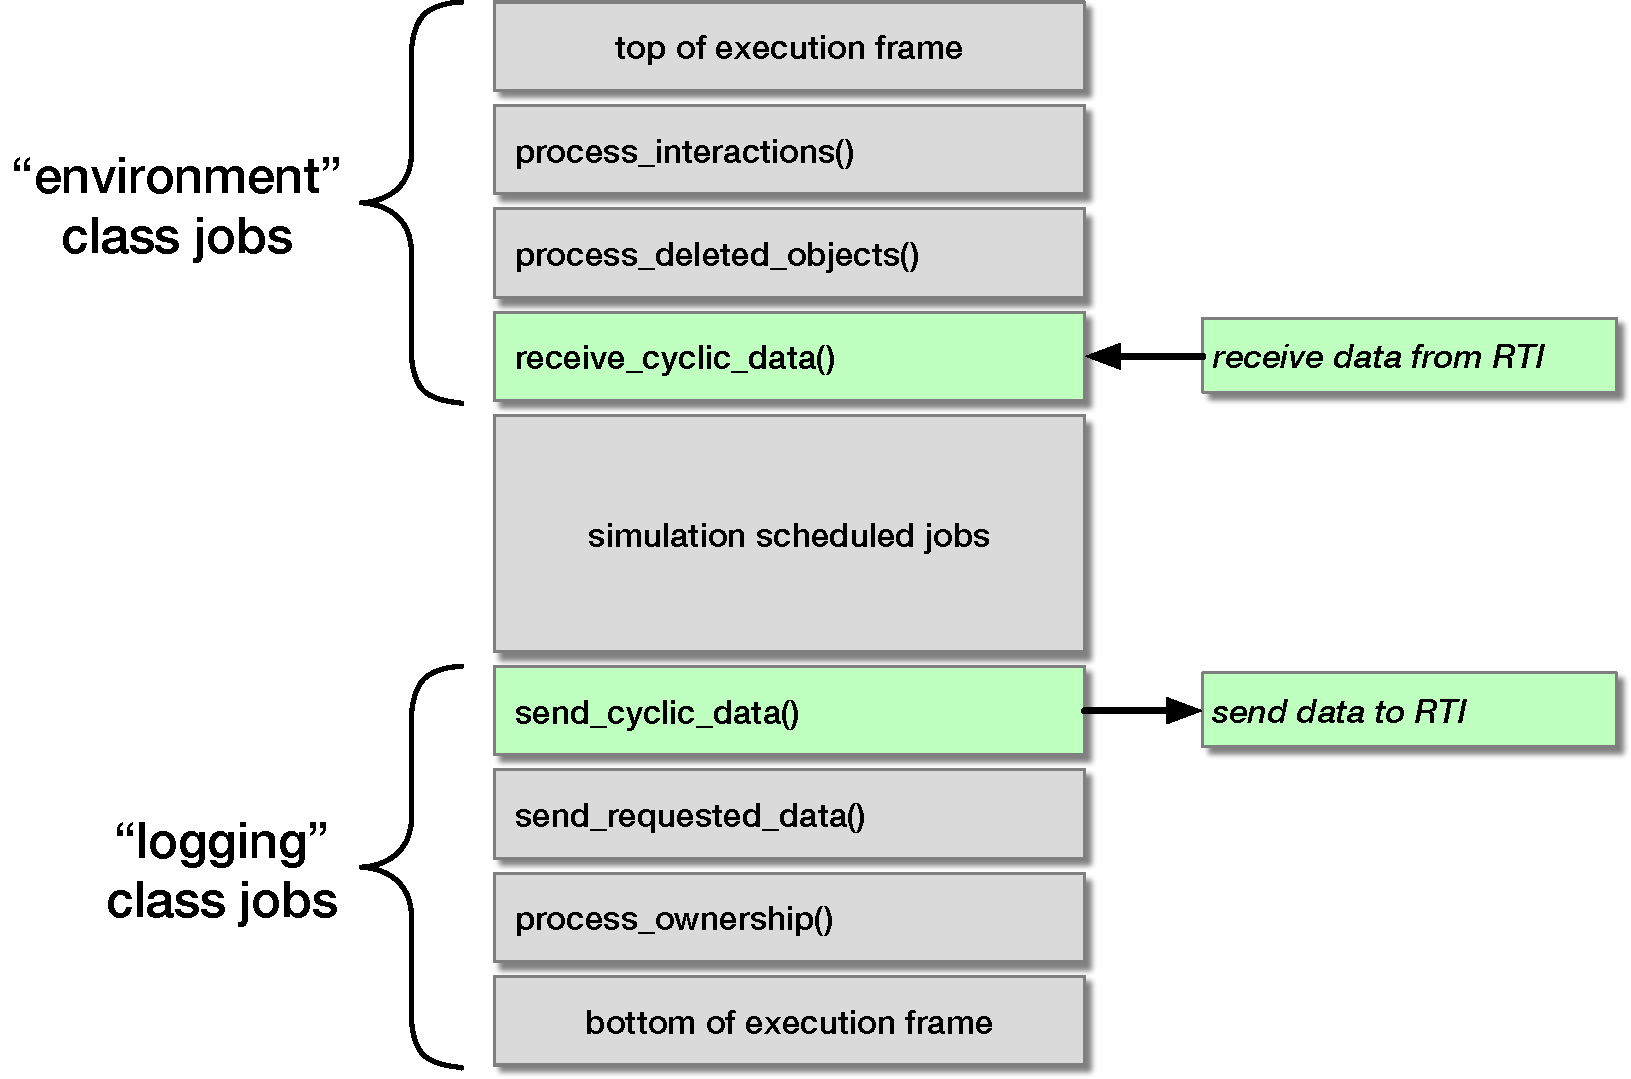
\includegraphics[scale=0.4]{TutorialTHLADataJobs.pdf}
      \end{figure}
   \end{frame}